


\documentclass[12pt, twoside, letterpaper]{book}

% GENERAL AUTHOR, TITLE AND KEYWORDS
%
% Nombre del Estudiante
\newcommand{\scriptAuthor}{Luis Roy Araya Núñez}

% Título de la tesis
\newcommand{\scriptTitle}{Desarrollo de Automatización de Selladora de Productos Médicos}

% Keywords
\newcommand{\scriptKeywords}{Sistema de Visión, Automatización, Diseño Mecánico, ...}

% Descripción de la editorial
\newcommand{\boxeditorial}{%
}

% Para el PDF (cambiar si se desea otras cosas a lo indicado arriba
\newcommand{\pdfAuthor}{\scriptAuthor}
\newcommand{\pdfTitle}{\scriptTitle}
\newcommand{\pdfKeywords}{\scriptKeywords}


\usepackage[utf8]{inputenc}
\usepackage[spanish]{babel}

\usepackage{float}
\usepackage{graphicx}

\usepackage{caption}
\usepackage{subcaption}

\graphicspath{ {imagenes/} }

\usepackage{amsmath}
\usepackage{amssymb,amstext}            % AMS-math and symbols package
\usepackage{mathrsfs}                   % Calygraphic fonts for transforms
\usepackage{array}                      % extensions to tabular environment
\usepackage{longtable}                  % supports extraordinary long tables
\usepackage{tabularx}                   % supports tables with fixed width
\usepackage{afterpage}                  % put something only after the page
\usepackage{multirow}                   % supports multiple row grouping in 
                                        % tables
\usepackage{multicol}                   % multiple columns environments
\usepackage{paralist}                   % a few enumeration settings
\usepackage{verbatim}

%\usepackage{fancyhdr}                   % fancy page headers

\usepackage{lastpage}


%Diagrama Gantt
\usepackage{pgfgantt}

%Poner pdfs
\usepackage{pdfpages}

%Margenes de pagina
\usepackage{geometry}
\geometry{letterpaper, margin=1.5in}

%Problemas de Quotes
\usepackage[autostyle=false, style=english]{csquotes}
\MakeOuterQuote{"}

% Use more than one optional parameter in a new commands
\usepackage{xargs}

% Coloured text etc.
\usepackage{xcolor}

%Links a imagenes y paginas
\usepackage{varioref}
\usepackage[linktocpage]{hyperref}
\usepackage{cleveref}

%para que el link vaya al inicio de la figura
\usepackage{caption}

%Eliminar cajas de hyperref y poner color a los links
\hypersetup{
    colorlinks,
    linkcolor={red!50!black},
    citecolor={blue!50!black},
    urlcolor={blue!80!black}
}

%TODO notes
\usepackage[colorinlistoftodos,prependcaption,textsize=tiny]{todonotes}

%Comandos para las notas
\newcommandx{\unsure}[2][1=]{\todo[linecolor=red,backgroundcolor=red!25,bordercolor=red,#1]{#2}}
\newcommandx{\change}[2][1=]{\todo[linecolor=blue,backgroundcolor=blue!25,bordercolor=blue,#1]{#2}}
\newcommandx{\info}[2][1=]{\todo[linecolor=OliveGreen,backgroundcolor=OliveGreen!25,bordercolor=OliveGreen,#1]{#2}}
\newcommandx{\improvement}[2][1=]{\todo[linecolor=Plum,backgroundcolor=Plum!25,bordercolor=Plum,#1]{#2}}
\newcommandx{\thiswillnotshow}[2][1=]{\todo[disable,#1]{#2}}
%

\title{PG}
\author{royaraya16 }
\date{July 2016}

\begin{document}

%\begin{titlepage}
%	\centering
%	
%	{\scshape\LARGE Tecnol\'ogico de Costa Rica \par}
%	\vspace{1cm}
%	{\scshape\Large \'Area Acad\'emica de Ingenier\'ia Mecatr\'onica \par}
%	\vspace{1.5cm}
%	
\includegraphics[width=0.5\textwidth]{tec.png}\par\vspace{2cm}
%	{\huge\bfseries Desarrollo de Automatizaci\'on de Selladora de Productos M\'edicos, Hologic, Inc.\par}
%	\vspace{2cm}
%	{\Large Luis Roy Araya N\'u\~nez, 201117227\par}
%	\vfill
	%supervised by\par
	%Dr.~Mark \textsc{Brown}

%	\vfill

% Bottom of the page
%	{\large \today\par}
%end{titlepage}

%\tableofcontents

%\newpage

%\listoftodos[Notes]

\newpage


\chapter{Introducci\'on}

\section{Contexto}

Fundada en 1985, \emph{Hologic, Inc} es desarrollador, fabricante
y distribuidor de productos de diagn\'ostico, sistemas de im\'agenes
m\'edicas y productos quir\'urgicos, con \'enfasis en atender a las necesidades de salud de las mujeres.
Con sede principal en Massachusets, la compa\~n\'ia opera cuatro unidades de negocio principales centradas en im\'agenes m\'edicas,
salud esquel\'etica, el diagn\'ostico de c\'ancer de mama, y salud ginecol\'ogica. 

Ofreciendo una completa gama de tecnolog\'ias y un s\'olido programa de investigaci\'on y desarrollo, Hologic
se ha comprometido a ayudar a las personas de todo el mundo pueden tener una vida m\'as
larga y saludable. \par

Hologic posee una amplia cartera de productos que ayudan a los m\'edicos a identi\'car
enfermedades en sus etapas m\'as tempranas, cuando las probabilidades de \'exito del tratamiento
est\'a en su m\'aximo. En el entorno sanitario desafiannte de hoy, Hologic se centra
en proporcionar a los clientes con tecnolog\'ias innovadoras que mejoran los resultados del
paciente e impulsan el rendimiento c\'inico, al tiempo que reduce al mismo tiempo los
costes sanitarios. \par

La sede de Hologic en Costa Rica se encarga principalmente del ensamble, pruebas, y
empaque de los dispositivos desechables utilizados para el diagn\'ostico de cancer de mama
y cirug\'ias ginecol\'ogicas, ver figura \ref{fig:Novasure}.

\begin{figure}[ht]
    \centering
    \begin{subfigure}[b]{0.45\textwidth}
        \centering
        
\includegraphics[width=\textwidth]{Novasure}
        \caption{Novasure}
        \label{fig:nova}
    \end{subfigure}
    \hfill
    \begin{subfigure}[b]{0.45\textwidth}
        \centering
        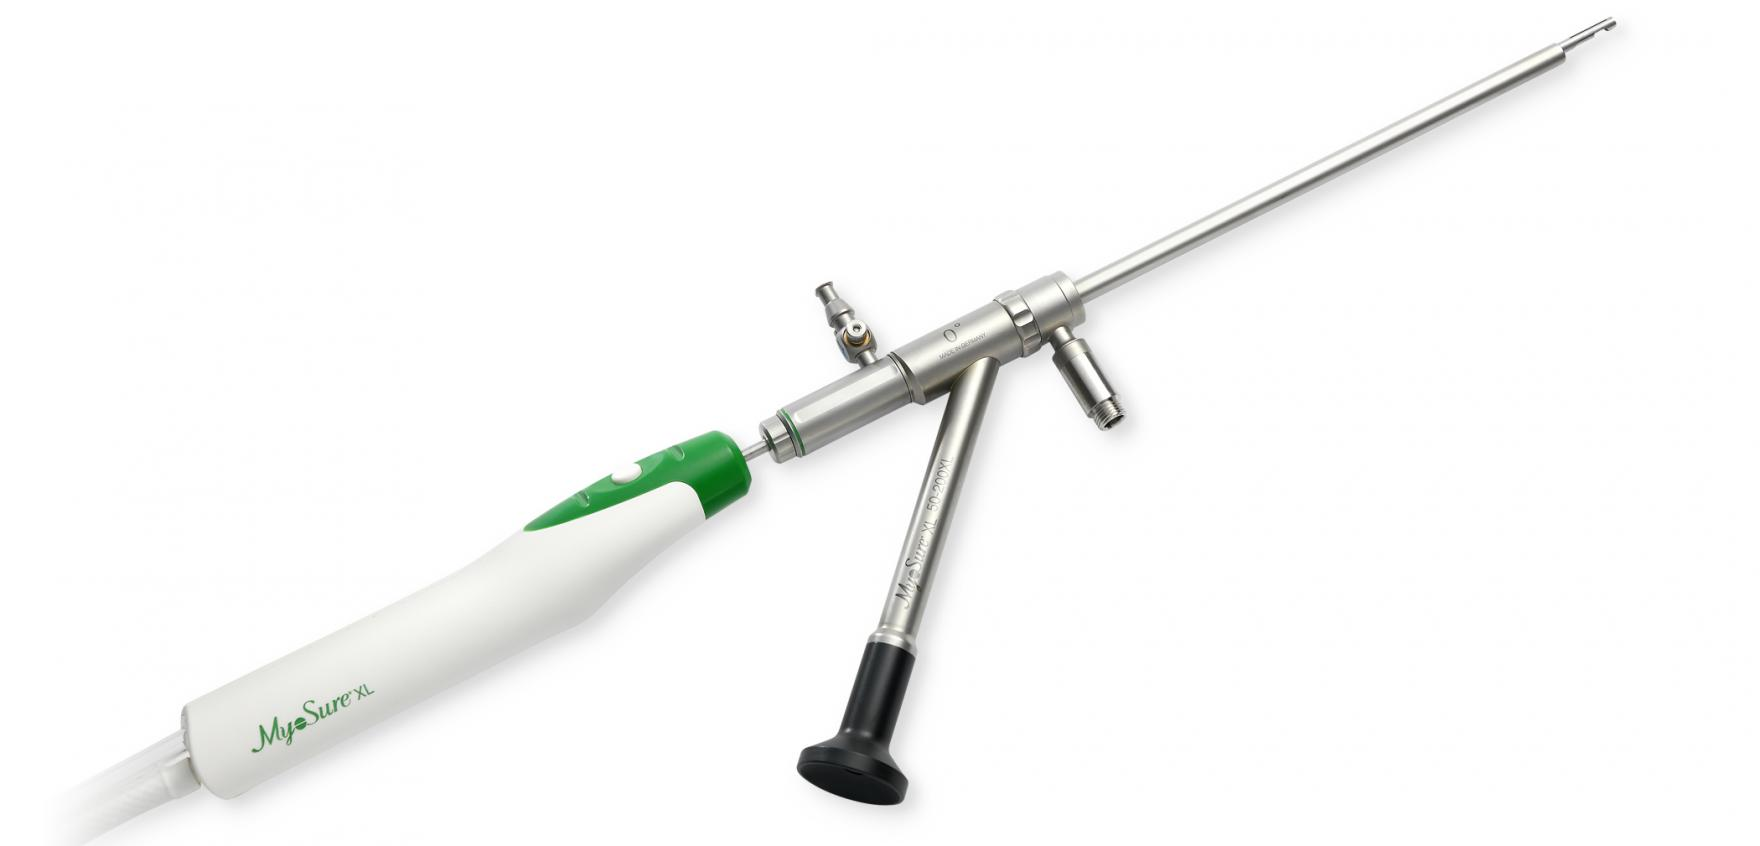
\includegraphics[width=\textwidth]{myosure}
        \caption{Myosure}
        \label{fig:myo}
    \end{subfigure}
    \caption{Dispositivos fabricado en Hologic Inc}
    \label{fig:Novasure}
\end{figure}


En el proceso de ensamble que se realiza en Costa Rica, las partes moldeadas se obtienen
de diferentes suplidores, para luego ser ensambladas en el cuarto limpio. El proceso de
ensamble es principalmente manual, con ayuda de peque\~nas m\'aquinas automatizadas para
posicionar, inspeccionar y probar el dispositivo. \par

Luego de que el dispositivo es completamente ensamblado pasa por una serie de pruebas
espec\'ificas que retan la funcionalidad del mismo. Se realizan pruebas de vac\'io, pruebas de esfuerzo a las piezas que se unen por medio de adhesivos, pruebas de continuidad
y resistividad a los componentes electr\'onicos, entre otros... \par


Luego se procede al empaque en el que se posicionan todos los componentes necesarios
para el m\'edico en un tray, semejante al que se observa en la figura \ref{fig:tray}.

\begin{figure}[H]
\centering
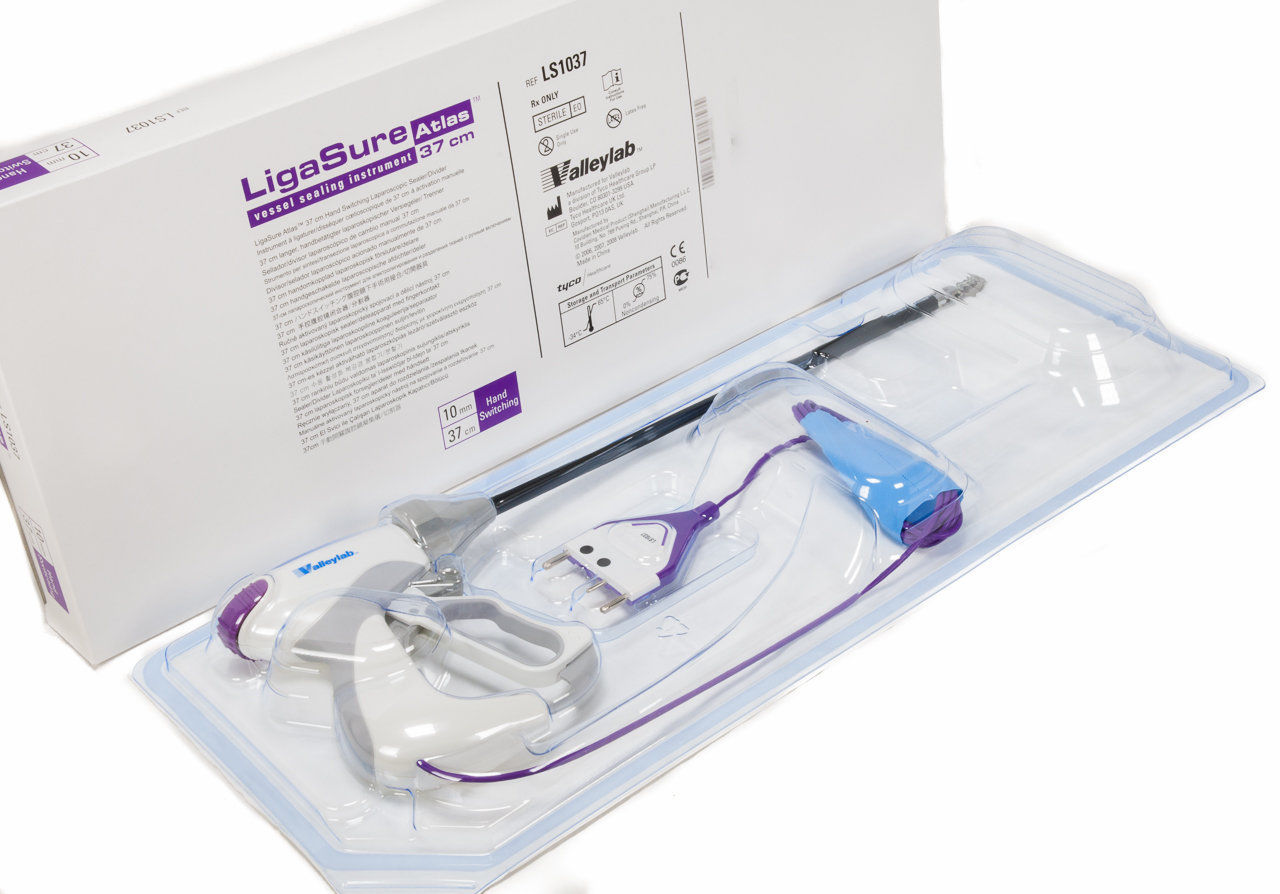
\includegraphics[width=0.5\textwidth]{trayImage}
\caption{Dispositivo en tray}
\label{fig:tray}
\end{figure}

Luego de que todos los componentes estan fijos dentro del tray, se procede al sellado. Luego del sellado se empacan los productos en cajas las cuales son enviadas a todo el mundo. Y con esto termina el proceso de fabricaci\'on producci\'on y env\'io.

\newpage
\section{Componentes faltantes en producto EVA}

El 10 de Mayo del 2013 fu\'e encontrado en el Laboratorio  de Control de Calidad, durante las pruebas Post Esterilizado en el producto EVA lote 13D10RB, un dispositivo sin una de sus partes, espec\'ificamente el insert, en la figura \ref{fig:insert} se puede observar que el insert es la pieza pl\'astica que se posiciona en la parte superior central, encargada de fijar el dispositivo al tray.

\begin{figure}[H]
\centering
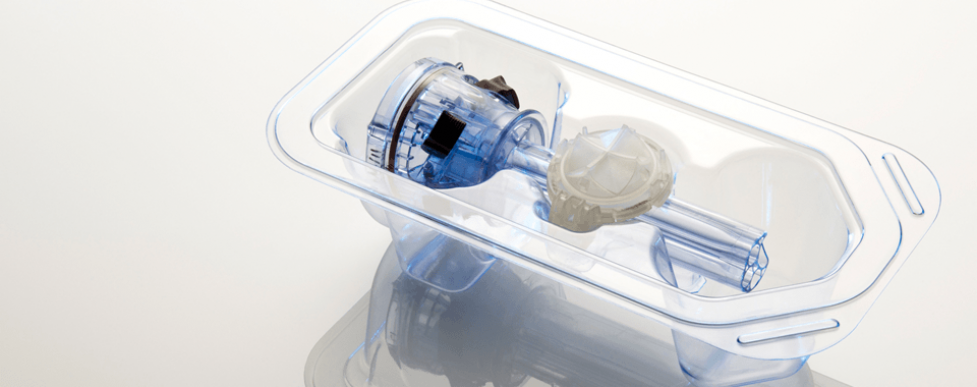
\includegraphics[width=0.8\textwidth]{trayInsert}
\caption{Ilustraci\'on de dispositivo enn el tray}
\label{fig:insert}
\end{figure}

Que esta pieza no est\'e podr\'ia ocasionar el da\~no del empaque, comprometiendo as\'i la integridad del esterilizado, parte vital en un dispositivo m\'edico.

Debido a este incidente en Junio del 2013 se abre una acci\'on correctiva (CAPA-00087) con el fin de eliminar este problema. Entre las acciones implementadas se encuentra la adici\'on en una de las estaciones de inspecci\'on un sensor para detectar el insert.

En Diciembre del 2013 se encuentran 3 unidades sin insert y adem\'as otra unidad con otro componente faltante, llamado introducer. Por esta raz\'on la acci\'on correctiva (CAPA-00087) se considera como inefectiva y el d\'ia 12 de Enero del 2014 se procede a levantar otra acci\'on correctiva (CAPA-00136).

En el CAPA-00136 se pretende investigar la causa ra\'iz del problema e implementar nuevas
acciones correctivas. Durante la investigaci\'on de la causa ra\'iz se concluye que algunas
unidades no completan el flujo de proceso completo, por lo que un componente faltante
podr\'ia ser pasado por alto. Una de las acciones correctivas aplicadas fue la adici\'on de
una estaci\'on de inspecci\'on del 100\% de las unidades despu\'es de la operaci\'on de sellado. Adem\'as, se implement\'o una forma sistem\'atica de asegurarse que las unidades completen el flujo de proceso requerido.

El 15 de Diciembre del 2014, durante la inspecci\'on de control de calidad del 100\% de
las unidades al final de la l\'inea de manufactura del producto EVA, fu\'e encontrada una
unidad con el insert faltante.

Esta anomalía se volvio a presentar al menos cuatro veces en un per\'iodo de seis meses y dado que la empresa en esta inspecci\'on requiere un 100\% de efectividad se levant\'o otra acci\'on correctiva (CAPA-00237), esta acci\'on fu\'e asignada al departamento de Fixtures \& Tooling.

El primer enfoque de soluci\'on que se trat\'o de implementar consist\'ia en aplicar una tinta invisible al tray durante la estaci\'on de insecci\'on,
esta tinta s\'olo ser\'ia visible por medio de la aplicaci\'on de una luz especial, la cual se encontrar\'ia dentro de la selladora,
con esto se pretend\'ia que la selladora revisara que todos los trays tuvieran la tinta, y de no ser as\'i no se procediera
con el sellado, ya que el tray que no tuviera la tinta invisible se habr\'ia saltado el \enquote{tray vision inspection system}.

Durante el a\~no se procedi\'o con la selecci\'on de componentes, el dise\~no mecanico, entre otras actividades.
Pero para Febrero del 2016 se recibieron resultados de pruebas qu\'imicas que se le realizaron a la tinta invisible que se planeaba
utilizar, los resultados mostraron componentes cancer\'igenos dentro de la tinta, por lo que su uso qued\'o totalmente descartado.

Desde esa fecha el proyecto se encuentra en hold, en la figura \ref{fig:timeline} se observa el tiempo que ha estado el problema sin una soluci\'on efectiva.

\begin{figure}[htb]
  \centering
  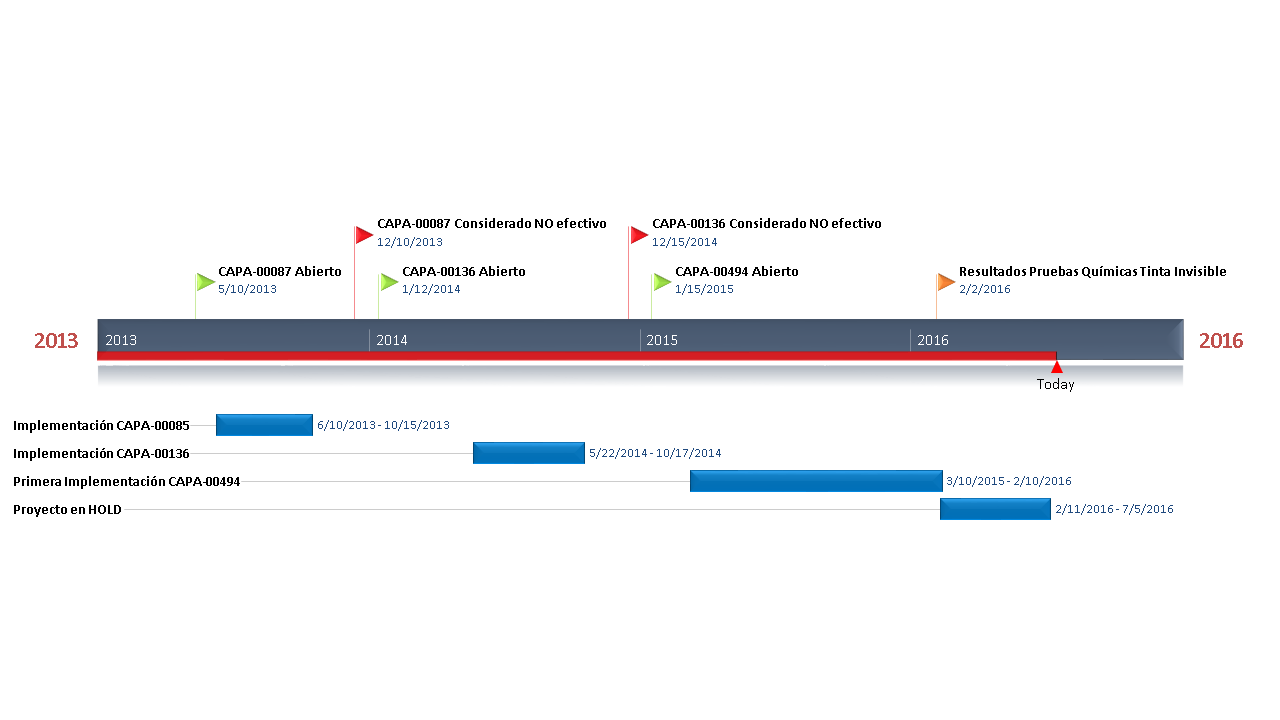
\includegraphics[width=0.9\textwidth]{timeline}
  \caption{L\'inea de tiempo}
  \label{fig:timeline}
\end{figure}


\subsection{An\'alisis de causa ra\'iz}
Para determinar la causa probable de la unidad con componentes faltantes durante la
inspecci\'on final se utiliza la siguiente herramienta de los 5 porqu\'es.

\begin{itemize}

    \item ¿Por qu\'e hay unidades EVA con componentes faltantes detectadas durante la inspecci\'on de control de calidad al final de la l\'inea de manufactura?
    
    Porque los componentes faltantes no fueron detectados durante el "tray vision inspection system" y la "Final Inspection". Como se observa en la figura \ref{fig:flowchart}, existen dos inspecciones antes de la inspecci\'on
    de control de calidad de 100\% que son capaces de detectar cualquier componente
    faltante en el dispositivo.
    
    \begin{figure}[H]
    \centering
    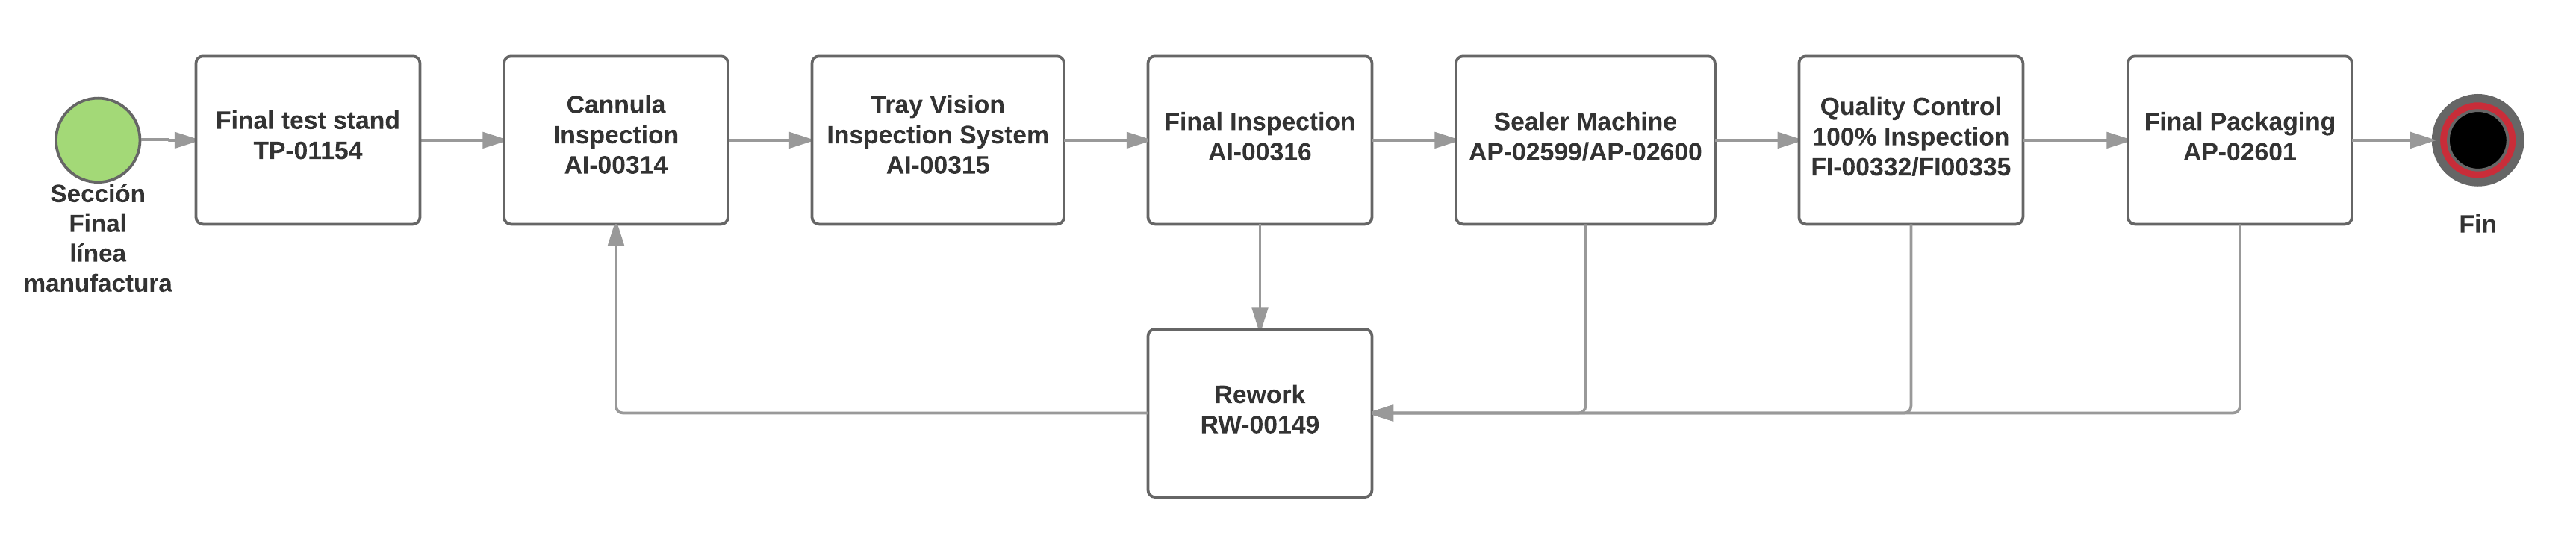
\includegraphics[width=1\textwidth]{flowchartEVA}
    \caption{Diagrama de flujo del proceso final de la l\'inea de manufactura}
    \label{fig:flowchart}
    \end{figure}
    
    \item ¿Por qu\'e no fueron detectadas las unidades con componentes faltantes durante el "tray vision inspection system" o la "Final inspection"?
    
    Porque algunas unidades (no intencionalmente) podr\'ian no estar realizando el flujo de proceso completo, evitando pasar por las inspecciones mencionadas anteriormente.
    
    La posibilidad de que la m\'aquina del "tray vision inspection system" no est\'e funcionando correctamente y acepte unidades incompletas es descartada debido a que
    estos equipos son validados para asegurar la confiabilidad de los mismos.
    
    \item ¿Por qu\'e hay unidades que no completan el flujo de proceso correcto? \par
    Debido a las siguientes situaciones:
    
        \begin{itemize}
        
            \item Situaci\'on 1: Si la cantidad de dispositivos en la estaci\'on de retrabajos es muy
            alta, es posible que se genere un error en el que la unidad pase directamente
            al sellado luego del retrabajo, ver figura \ref{fig:incorrectFlow}. La l\'inea roja representa el flujo
            incorrecto que algunas unidades podr\'ian estar experimentando.
            
            \item Situaci\'on 2: Durante el proceso de "Tray vision inspection system" el operario podr\'ia pasar un dispositivo incompleto a la siguiente estaci\'on, omitiendo la alarma de fallo del equipo.
        
        \end{itemize}
        
    \begin{figure}[ht]
    \centering
    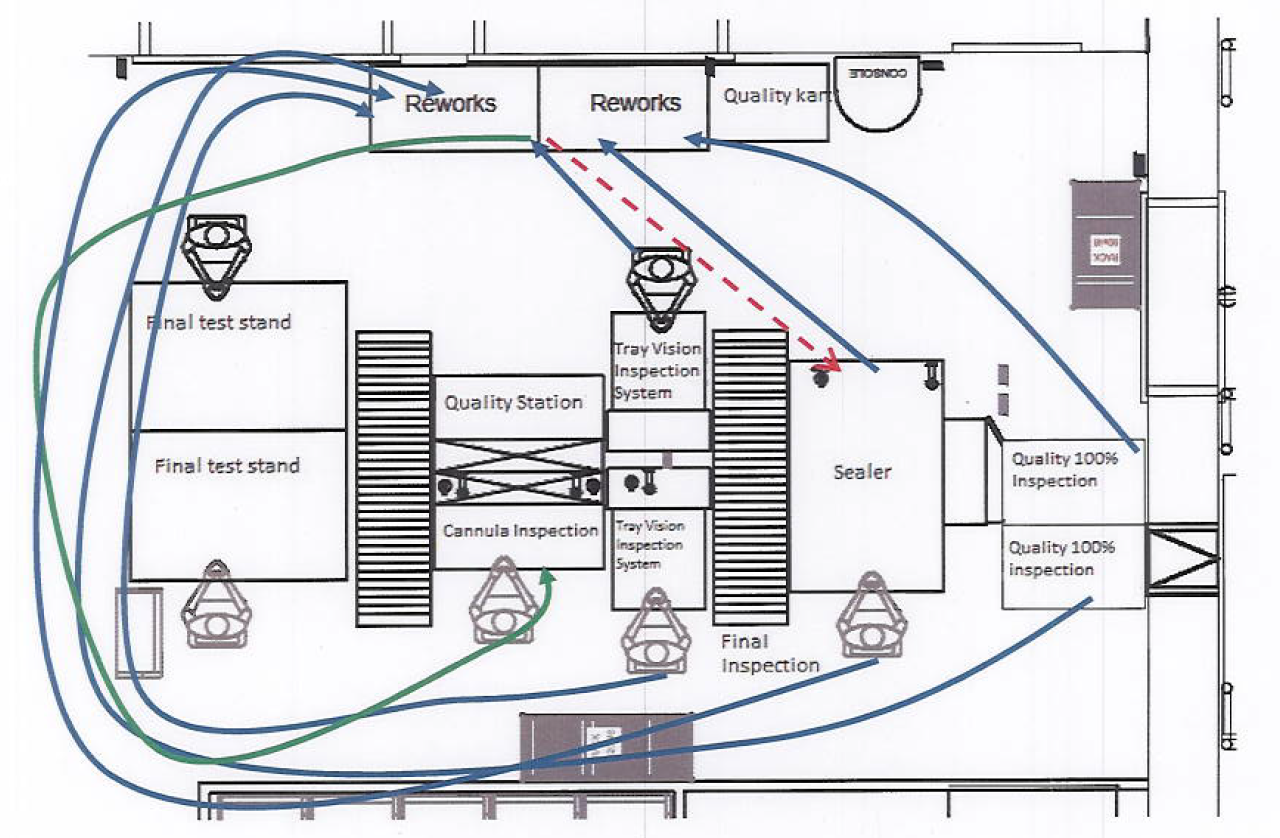
\includegraphics[width=1\textwidth]{incorrectFlowProccess}
    \caption{Flujo incorrecto de proceso}
    \label{fig:incorrectFlow}
    \end{figure}
    
    \item ¿Por qu\'e ocurren las situaciones anteriores en la l\'inea de manufactura del producto
    EVA?
    
    \begin{itemize}
    
        \item Situaci\'on 1: La cantidad de dispositivos en retrabajos es alta debido a que
        durante las inspecciones visuales que se realizan como parte del procedimiento
        muchas veces se encuentran part\'iculas indeseadas, estas part\'iculas provienen
        principalmente de una de las partes de un suplidor espec\'ifico, el cual ya fue
        contactado. Adem\'as, el flujo correcto que deben seguir las unidades luego de los
        retrabajos no es\'ta claramente documentado ni explicado en los procedimientos.
        
        \item Situaci\'on 2: La inspecci\'on por medio del sistema de visi\'on que existe actualmente algunas veces brinda falsos positivos, esto significa que el equipo alerta que falta un componente, pero en realidad si est\'a presente. Esto ocurre debido al posicionamiento incorrecto del dispositivo dentro del tray. En estos casos
        el operador desbloquea el equipo y realiza una inspecci\'on visual para pasar el
        dispositivo a la siguiente estaci\'on.
    
    \end{itemize}

\end{itemize}


\subsection{Causa Ra\'iz}
Picos de alta incidencia de retrabajos pueden inducir a un error que evite la verificaci\'on de componentes faltantes en el dispositivo.

\subsection{Factores Contribuyentes}

\begin{itemize}

    \item Falta de control en el sistema de inspecci\'on, ya que permite que el operador pueda pasar unidades sin la aprobaci\'on del sistema.
    
    \item Falta de instrucciones claras y documentadas que definan el flujo de proceso requerido para las unidades.

\end{itemize}

\subsection{S\'intesis del problema}
Componentes faltantes en el producto EVA durante la inspecci\'on al final de la l\'inea de manufactura

\newpage
\section{Enfoque de la soluci\'on}

%\subsection{Criterios de selecci\'on de la soluci\'on}

%A continuaci\'on, se presenta una lista con los criterios de selecci\'on de la soluci\'on:

%\begin{itemize}

%    \item Presupuesto
%    \item Complejidad
%    \item Tiempo de Ejecuci\'on
%    \item Confiabilidad

%\end{itemize}

\subsection{Soluci\'on Propuesta}

La soluci\'on que se propone consiste en la integraci\'on de tres de los puestos que se tienen actualmente, los cuales ser\'ian el "tray inspection vision system", "Final Inspection" y "Sealer Machine", ver figura \ref{fig:solution}. \par

La idea es realizar una modificaci\'on a la selladora para que en la misma se encuentre el sistema de inspecci\'on, el cual consiste en la detecci\'on de cuatro componentes del producto EVA, los cuales son:

\begin{itemize}

    \item Insert
    \item Introducer
    \item Stylet
    \item Scoop

\end{itemize}

De los cuatro componentes anteriores, el Insert, Introducer y Stylet se inspeccionar\'an por medio de un sistema de visi\'on, el cual se compondr\'ia de seis c\'amaras. La cantidad de productos que se pueden sellar en una operaci\'on. El cuarto componente consiste en una peque\~na parte met\'alica, por lo que se utilizar\'a un sensor inductivo para su detecci\'on, la detecci\'on del Scoop por medio de las c\'amaras es descartada debido a que la pieza met\'alica se encuentra dentro de un encapsulado pl\'astico. \par

Las c\'amaras se comunicar\'ian con el PLC existente en la selladora por medio de salidas digitales, las cuales representan el estado de la inspecci\'on (PASS/FAIL). El resultado de la inspecci\'on se desplegar\'a en una pantalla HMI en tiempo real. \par

La m\'aquina de sellado que actualmente se utiliza en la l\'inea se opera de forma manual, una automatizaci\'on de la misma es necesaria para poder eliminar el error humano. Por lo tanto, se a\~nadir\'an actuadores neum\'aticos los cuales mover\'an los nidos que contienen los productos hacia la plancha caliente que realiza el sellado. \par

Para eliminar por completo alguna perturbaci\'on por parte del operario en el producto se implementar\'an cortinas de luz, las que se utilizan normalmente en aplicaciones de seguridad. Su aplicaci\'on ser\'ia principalmente para sensar si el operario tiene contacto con el producto una vez que ya est\'a puesto en los nidos para sellar. El accionamiento de la m\'aquina de sellado ser\'a por medio de un bot\'on, el cual justo despu\'es de su accionamiento active la inspecci\'on y si y s\'olo si la inspecci\'on es exitosa se realice el sellado, de lo contrario se deber\'a entrar en estado de error e informar al operario de los componentes faltantes.

\subsection{Factibilidad de la soluci\'on propuesta}

La soluci\'on propuesta presenta un gran ahorro tanto en tiempo de manufactura, como en devoluciones a los clientes ya que por cada unidad incompleta se debe enviar otra sin costo adicional, adem\'as se asegura que el sellado se realice s\'olo con unidades completas sin intervenci\'on humana. \par

Con la reducci\'on del tiempo de manufactura se tiene que las dos operaciones que se eliminar\'ian juntas poseen un tiempo est\'andar de aproximadamente $1.5$ minutos. El tiempo de manufactura total del producto se encuentra por $14$ minutos, $23$ segundos.  \par

Con estos datos se puede decir que la implementaci\'on de la propuesta reducir\'ia en aproximadamente un 10\% el tiempo de manufactura de cada producto. Tambi\'en al eliminar esas dos operaciones se ahorran dos recursos del departamento de calidad. \par

En cuanto al ahorro por devoluciones, se estima que cada mes se realizan al menos 5 devoluciones por componentes faltantes. El precio de cada dispositivo ronda los \$800, por lo que se tendr\'ia un ahorro estimado, con respecto a las devoluciones de \$4 000 mensuales.

\begin{figure}[H]
\centering
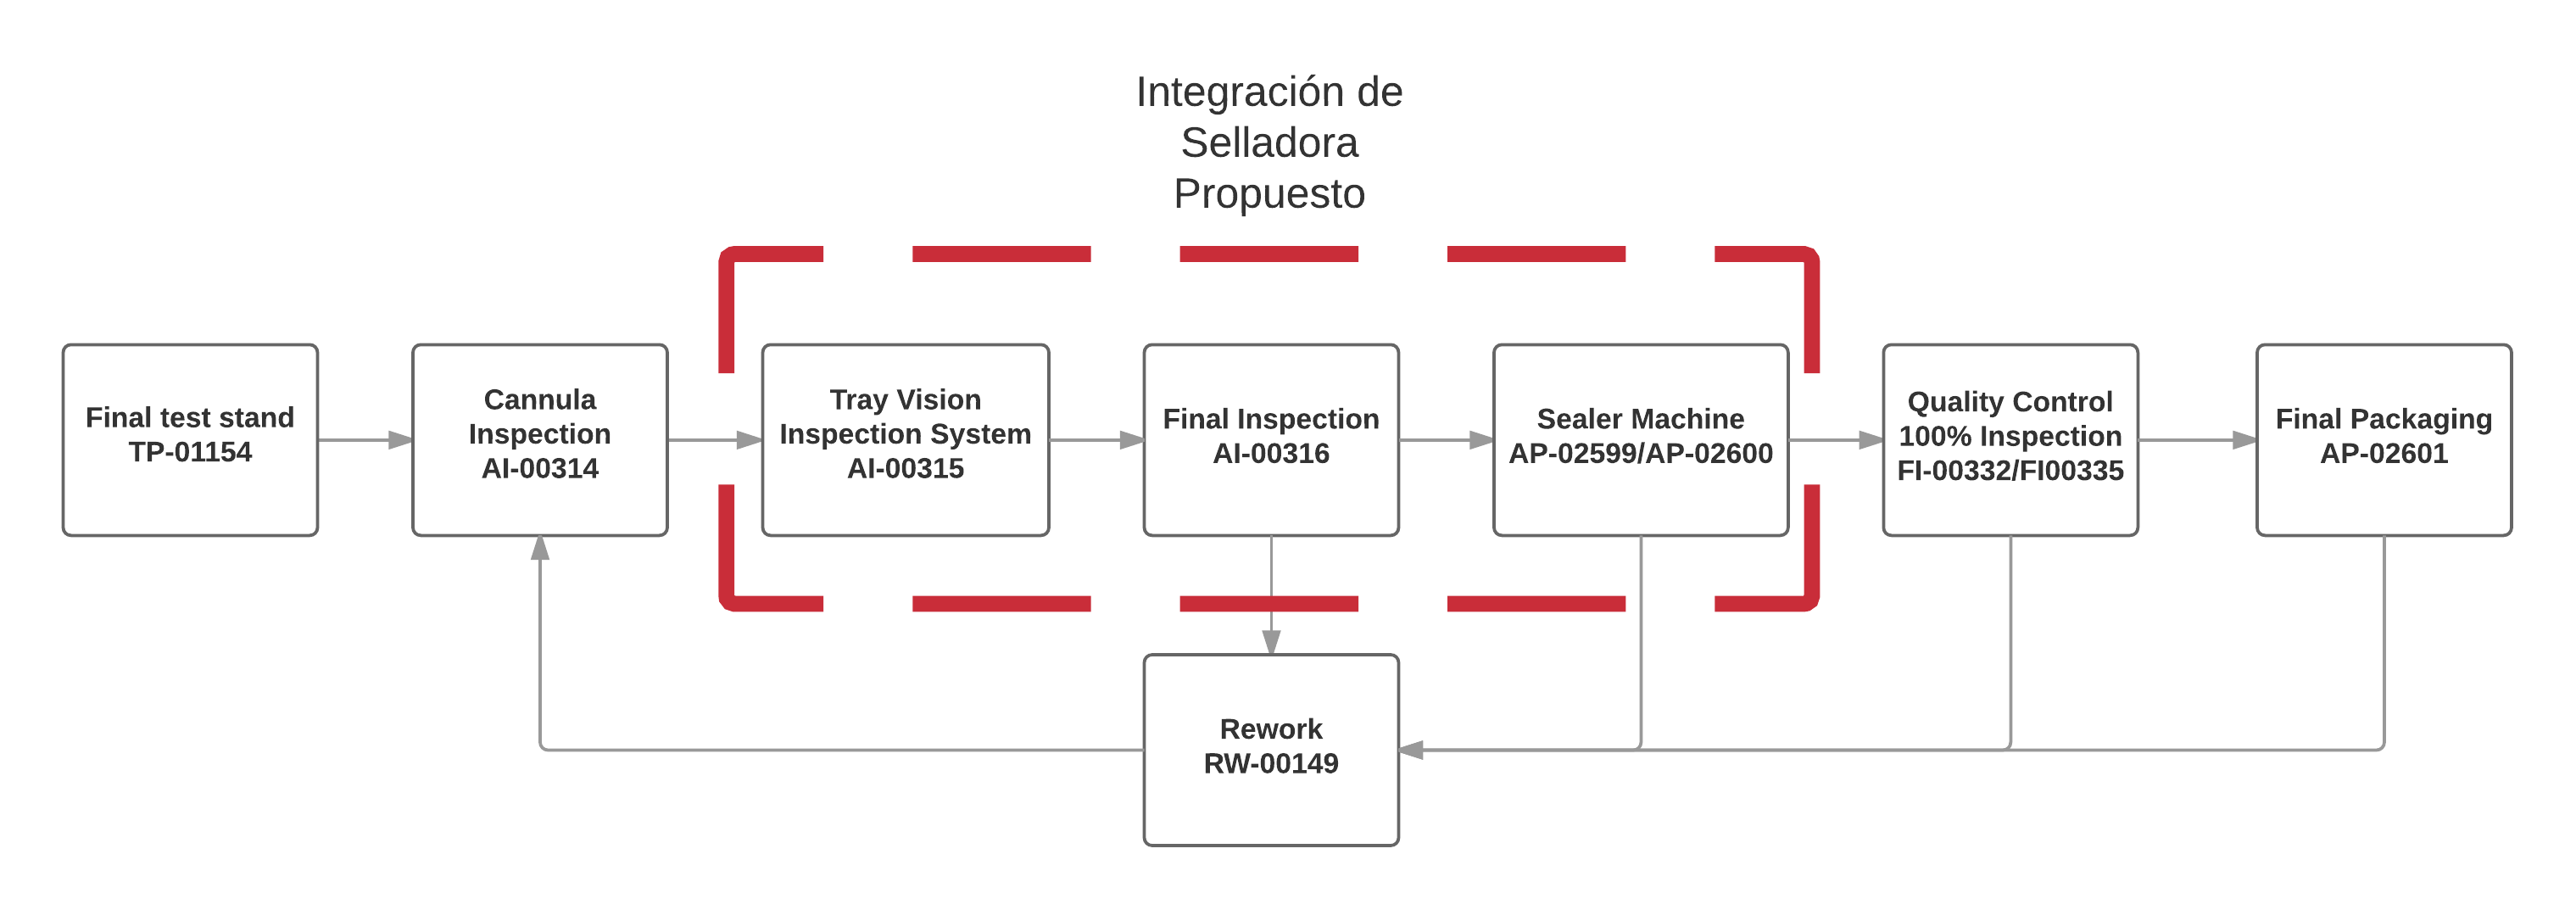
\includegraphics[width=1\textwidth]{flowchartPropuesto}
\caption{Soluci\'on propuesta}
\label{fig:solution}
\end{figure}


\newpage
\section{Objetivos}

\subsection{Objetivo general}

\begin{itemize}

\item Desarrollar un sistema integrado de inspecci\'on y sellado del producto EVA,
que no permita el sellado de unidades incompletas.

%\textbf{Indicador:} Sellado de un 100\% de unidades completas durante la operaci\'on integrada de inspecci\'on y sellado.

\end{itemize}

\subsection{Objetivos espec\'ificos}

\begin{itemize}

    \item Crear un sistema de visi\'on que detecte la presencia del insert, introducer
    y stylet dentro del producto EVA.
    
    %\textbf{Entregable:} Algoritmo de detecci\'on de los componentes deseados, en el que nunca se presente un falso positivo, esto significa que en ning\'un momento el algoritmo debe retornar la existencia de una pieza que en realidad no se encuentra.
    
    \item Proponer las modificaciones mec\'anicas necesarias en la selladora para
    la integraci\'on del sistema de visi\'on.
    
    %\textbf{Entregable:} Planos Mec\'anicos de modificaciones que aislen cualquier interveci\'on humana en el producto durante el sellado y que al mismo tiempo cumpla con los requisitos de espacio, automatizaci\'on y posicionamiento de las c\'amaras, permitiendo una integraci\'on sin errores o complicaciones.
    
    \item Integrar el sistema de visi\'on y las modificaciones mec\'anicas en la
    m\'aquina de sellado.
    
    %\textbf{Indicador:} Funcionamiento con 100\% de efectividad de la m\'aquina de sellado, integrando correctamente la automatizaci\'on de la m\'aquina junto con la inspecci\'on por medio del sistema de visi\'on.

\end{itemize}

\chapter{Marco Te\'orico}

Enumeracion de las diferentes partes del marco teorico

\begin{itemize}
    \item Sistema de vision, smart Cameras
    \item FOV, ROI, Iluminacion, Backlight
    \item Algoritmo utilizado, FAST
    \item Sensores, Cortinas de Luz, Seguridad Tipo 4
    \item Piston, Seleccion, Valvulas centro cerrado
    \item Dise\~no Mec\'anico, Perfiles ALuminio Modulares
    \item Automatizacion, PLC, HMI
     
\end{itemize}

%\newpage
%\section
%\section{Referencias}

%\begin{thebibliography}{plain}

%\bibitem{a} Wilson, W. M. (1997). Writing Effective Requirements Specifications.
%Software Technology Conference \par

%\bibitem{b} INCOSE. (2015). Systems Engineering Handbook: A Guide for System
%Life Cycle Processes and Activities. San Diego: Wiley \par

%\bibitem{c} Project Management Institute (2013). A Guide to the Project Managemente
%Body of Knowlege (5 ed.) Pa:Newtown Square



\bibliographystyle{unsrt}
\bibliography{mendeley}

%\end{thebibliography}

\end{document}
